\ifdefined\XeTeXversion\RequirePackage[T1]{fontenc}\fi
\documentclass[conference]{IEEEtran}
\usepackage[T1]{fontenc}
\usepackage{balance}
\usepackage{cite,amsmath,amssymb,graphicx,booktabs,array,tabularx}
\usepackage{tikz}
\usetikzlibrary{arrows.meta,positioning,fit}
\usepackage{listings}
\usepackage[hyphens]{url}
\usepackage[hidelinks]{hyperref}
\urlstyle{same}
\newcolumntype{Y}{>{\raggedright\arraybackslash}X}
\lstset{basicstyle=\ttfamily\scriptsize,breaklines=true,columns=fullflexible,
 frame=single,aboveskip=6pt,belowskip=6pt,showstringspaces=false}
\tikzset{box/.style={draw,rounded corners=1pt,align=center,font=\scriptsize,
 minimum height=7mm,inner sep=2pt,text width=22mm},arr/.style={-{Latex[length=1.5mm]},thin}}
\newcommand{\code}[1]{\texttt{#1}}
\hyphenation{PostgreSQL RabbitMQ PayOS Flutter}
\begin{document}
\title{CosmoQ Cinema: A Cross-Platform Flutter Mobile Ticket Booking Application with an ASP.NET Core Backend}
\author{
\IEEEauthorblockN{Nguyen Nguyen Ngu (QE190064), Dao Thi Thanh Huong (QE190046),\\
Pham Ngo Bich Tram (QE1900100), Nguyen Hoang Ngoc Chau (QE190088),\\
Nguyen Xuan Dang Khoa (QE1900126)}
\IEEEauthorblockA{Student Developers, Class: SEK19B.Net\\
Department of Software Engineering\\
FPT University Quy Nhon Campus, Binh Dinh, Vietnam}
\IEEEauthorblockN{Huynh Vang}
\IEEEauthorblockA{Project Advisor, Lecturer, Department of Software Engineering\\
FPT University Quy Nhon Campus, Binh Dinh, Vietnam\\
vangh@fe.edu.vn}}
\maketitle
\begin{abstract}
Mobile cinema booking must coordinate local screen state with server-owned
reservations while users leave the application for payment and later return.
CosmoQ Cinema addresses this workflow with a Flutter customer application and
a shared ASP.NET Core 8 backend behind a YARP gateway. This report examines
the mobile implementation using startup code, navigation, remote repositories,
HTTP adapters, platform configuration, SQL, and tests. The client uses explicit
session notifications, secure-storage calls, coordinated refresh-token renewal,
movie/showtime discovery, periodically updated seat maps, booking history,
and QR ticket presentation. The backend uses Entity Framework Core and Npgsql
with PostgreSQL, server-priced ten-minute holds, PayOS verification, and
RabbitMQ-mediated notification and refund processing. Mobile-specific paths
include external checkout, application-resumption verification, ticket sharing,
calendar URLs, and staff QR-scanner integration. The analysis distinguishes
these source implementations from successful physical-device execution.
Seventeen isolated booking-service tests and twenty-one gateway tests passed;
backend builds succeeded with four MovieService nullable warnings. The Flutter suite passed 209 tests, with one informational analysis lint.
Docker-backed integration was blocked, and native release, live merchant payment, and device
acceptance were not executed. The report contributes an evidence-linked
description of mobile state recovery and booking coordination without treating
plugin dependencies, test doubles, or platform folders as proof of operational
completion.
\end{abstract}
\begin{IEEEkeywords}
Mobile ticket booking, Flutter, Dart, ASP.NET Core, JWT, PostgreSQL, PayOS, QR tickets.
\end{IEEEkeywords}

\section{Introduction}
Mobile cinema booking brings discovery, seat choice, payment, and ticket access
into a small-screen interaction. The user may leave the application to pay,
return after the operating system pauses it, or revisit a booking after a
network failure. A client must preserve an understandable distinction between
local selection, a server-held reservation, and a paid ticket. CosmoQ Cinema
addresses these tasks through a Flutter customer application connected to a
shared ASP.NET Core backend \cite{client,booking}.

This paper focuses on the mobile build of the customer entry point in
\code{Cinema\_Mobile}. The repository also builds browser applications, but
their management workspace is not a principal topic here. Platform directories
exist for Android and iOS, as well as desktop targets; directory presence is
not evidence that every platform has been built, signed, deployed, or tested.
The verified source supports discussing a cross-platform implementation while
retaining those distinctions.

The project's engineering contribution is a coordinated customer workflow:
remote catalog data, route-driven screens, recoverable authentication,
server-controlled seat holds, external PayOS checkout, booking history, and QR
ticket presentation. Notification read state, promotions, loyalty points,
reviews, ticket sharing, and a staff check-in path extend that workflow.
The contribution is the integration of these mechanisms in the inspected
project, rather than a novel mobile framework or a measured improvement over
existing cinema applications.

\subsection{Inspection Method and Claim Boundaries}
Source revision \code{55642353331f} and database revision
\code{e455d297c76b} define the inspected snapshot on October 28, 2026.
Inspection traced startup, routes, repositories, HTTP adapters, storage,
platform manifests, backend controllers/services, SQL constraints, tests, and
CI configuration. Requirements documents were not treated as proof of finished
behavior. The technology references explain APIs; repository citations identify
CosmoQ's implementation decisions.

The report separates strong implementation evidence from successful device
execution. Real HTTP repositories are selected by startup, while fake
repositories are used in tests. A source-level PayOS integration is not evidence
that a mobile customer completed a banking transaction. Likewise, use of a
secure-storage package is not a claim that storage and permissions were
validated on every supported operating system. Section VII describes what was
actually compiled, executed, or blocked.

\section{System Architecture Overview}
\subsection{Mobile-to-Service Topology}
The mobile application uses the same public API gateway as the other client
builds. It serializes requests as JSON and adds a bearer token for protected
operations. The gateway forwards requests to AuthService, MovieService, or
BookingService. Backend dependencies include PostgreSQL and RabbitMQ; external
communication includes PayOS HTTP calls and SMTP email. Figure~\ref{fig:architecture}
shows these boundaries from the mobile customer's perspective
\cite{client,gateway,deployment}.
\begin{figure}[t]
\centering
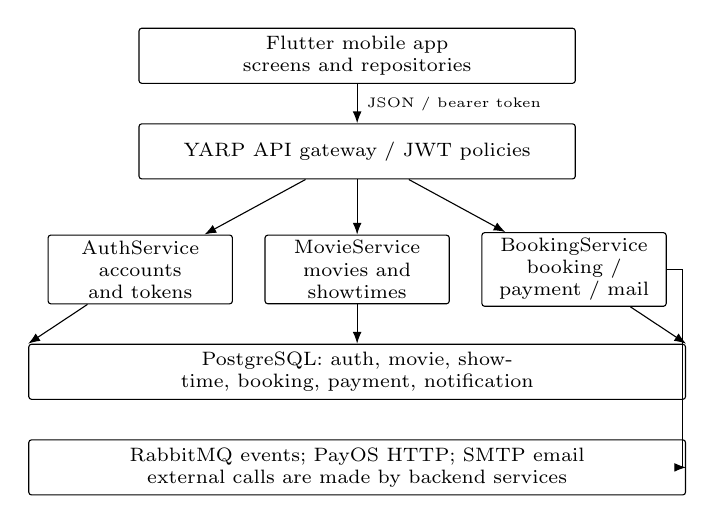
\begin{tikzpicture}[node distance=5mm and 4mm]
\node[box,text width=54mm] (ui) {Flutter mobile app\\screens and repositories};
\node[box,below=of ui,text width=54mm] (gw) {YARP API gateway / JWT policies};
\node[box,below=7mm of gw] (mo) {MovieService\\movies and showtimes};
\node[box,left=of mo] (au) {AuthService\\accounts and tokens};
\node[box,right=of mo] (bo) {BookingService\\booking / payment / mail};
\node[box,below=of mo,text width=82mm] (db) {PostgreSQL: auth, movie, showtime, booking, payment, notification};
\node[box,below=of db,text width=82mm] (ext) {RabbitMQ events; PayOS HTTP; SMTP email\\external calls are made by backend services};
\draw[arr] (ui)--node[right,font=\tiny]{JSON / bearer token}(gw);
\draw[arr] (gw)--(au);\draw[arr] (gw)--(mo);\draw[arr] (gw)--(bo);
\draw[arr] (au)--(db.north west);\draw[arr] (mo)--(db);\draw[arr] (bo)--(db.north east);
\draw[arr] (bo.east) -- ++(2mm,0) |- (ext.east);
\end{tikzpicture}
\caption{Selected deployment overview. Requests enter the gateway; services
access their database contexts. The bottom box groups backend integrations.}
\label{fig:architecture}
\end{figure}


There are three domain-service executables plus the gateway. MovieService also
contains showtime and room code; BookingService contains payment and
notification code. These modules are not separate deployed services merely
because they have their own classes or database contexts. The gateway and
services are individually defined in Docker Compose, which provides a local
service-based topology rather than evidence of an operational cloud platform.

\subsection{Verified Technology Stack}
Table~\ref{tab:stack} distinguishes client, backend, and integration technology.
The client uses Material widgets and Dart's asynchronous futures; no active
Bloc or Riverpod implementation was needed to explain its state flow.
Flutter's architecture documentation is relevant context \cite{flutter}, but
the classes actually instantiated by \code{AppDependencies.remote} determine
CosmoQ's behavior \cite{client}.
\begin{table}[t]
\caption{Verified Mobile Technology Stack}\label{tab:stack}
\centering\footnotesize
\begin{tabularx}{\columnwidth}{@{}lYY@{}}\toprule
Component & Technology & Responsibility\\\midrule
Mobile UI & Flutter, Dart, Material & Customer screens and navigation\\
Networking & Dart \code{http} & JSON requests and error handling\\
Session storage & \code{flutter\_secure\_}\allowbreak\code{storage} & Persist tokens and user data\\
Platform actions & \code{url\_launcher}, \code{share\_plus} & Checkout, links, sharing\\
Tickets & \code{qr\_flutter}, \code{mobile\_scanner} & QR display and staff scanning\\
Shared backend & ASP.NET Core 8; YARP & Identity, catalog, booking APIs\\
Data access & EF Core 8 and Npgsql & Six PostgreSQL databases\\
Events/payment & RabbitMQ; PayOS & Async follow-up and checkout\\\bottomrule
\end{tabularx}
\end{table}

The locally installed SDK reports Flutter 3.47.2 and Dart 3.13.2, matching the
manifest's Dart range. CI requests Flutter 3.47.4. Backend targets are .NET 8
and the review host uses .NET SDK 9.0.305. These version facts describe the
review and configuration; they do not assert a version for a published mobile
release \cite{tests,client}.

\subsection{Configuration and Data Flow}
\code{ApiConfig} defaults Android's emulator connection to
\code{http://10.0.2.2:5000}; other default targets use localhost. A physical
phone requires an appropriate \code{API\_BASE\_URL} build definition and network
access to the gateway. A payment return URL can also be overridden. Defaults
for local development should not be read as HTTPS deployment evidence
\cite{client,deployment}.

The UI calls repository interfaces, whose remote implementations invoke service
adapters and a shared HTTP client. JSON models hold movies, showtimes, seats,
bookings, payments, notifications, and authentication data. The repositories
combine data when a screen requires more than one backend resource: seat
layout comes from MovieService and occupied IDs from BookingService. This is
client-side composition of server results, not direct database access.

\section{Backend Design and Implementation}
\subsection{Identity as a Mobile Session Dependency}
AuthService supports email registration and OTP verification, login, refresh,
logout, password recovery, and profile/password changes. BCrypt hashes
passwords and OTP values; JWTs carry the user's identity and role claims.
JWT signing is HMAC-SHA256. The refresh flow revokes an accepted old refresh
token before returning new session credentials. Tokens originate in this
service rather than in a social-login or federated identity provider
\cite{auth}.

For the phone, the useful contract is an authentication response followed by
authenticated API requests and recovery from expiry. Issuer, audience,
signature, and lifetime checks occur in gateway/service JWT validation.
Gateway middleware also requests current account status for protected
requests. A locked account or changed roles can therefore invalidate continued
use through the gateway even while a token's timestamp is still valid. An
unreachable status service results in 503, which the mobile client must present
as a service failure rather than a successful action \cite{gateway,jwt}.

\subsection{Catalog and Seat Information}
MovieService supplies browsing, details, genres, and showtime selection. The
showtime implementation checks that selected seats belong to the showtime's
room, the show is open, and its start time is still in the future. Sweetbox
seats are validated as pairs when the partner is defined. These checks run
server-side independently of the phone's selection widgets \cite{movie}.

Seat pricing uses a format surcharge followed by a type surcharge. Normal,
VIP, and sweetbox values are defined in helpers; the resulting seat prices
are returned in server responses and reobtained for booking creation. The
mobile display helps the user understand a total, while the backend supplies
the authoritative amount. This limits trust in stale or manipulated client
inputs without asserting that every possible pricing scenario was device-tested.

\subsection{Reservation Lifecycle}
On booking submission, BookingService validates the request, rejects repeated
seat IDs, prices concessions from its menu, resolves promotions, and applies
permitted loyalty redemption. Customer identity is taken from claims by the
controller. The service records the showtime time received from MovieService;
movie title retrieval includes a request-title fallback if the remote lookup
returns no title \cite{booking}.

The reservation transaction locks existing seat/showtime records with
\code{FOR UPDATE}. It rejects booked seats and active holds, creates a pending
booking with a ten-minute expiry, and associates held seats. The unique
\code{(showtime\_id, seat\_id)} key handles competing inserts when a reservation
row has not existed before. A unique-violation exception is translated into a
conflict response. The phone cannot turn a locally highlighted seat into a
reservation until this transaction succeeds \cite{booking,db,postgres}.

A background expiry worker changes overdue pending bookings and releases their
seat holds. Payment confirmation attempts to transition the booking to a paid
state, while cancellation and refund paths have distinct rules. In particular,
a paid customer cancellation request can become \code{REFUND\_PENDING}; it
does not simply free the seats before the refund decision. This distinction
must remain visible in booking history rather than being reduced to a
client-side Boolean \cite{booking}.

\subsection{Database Design for Mobile Workflows}
SQL initialization creates six databases on the configured PostgreSQL 17
instance. Auth data uses users, roles, a join table, refresh tokens, and OTPs.
Movie data is separate from rooms, seats, and showtimes. Booking data includes
seat snapshots, reservations, concessions, promotions, loyalty records, and
reviews. Payment and notification records have separate contexts/databases.
The Npgsql EF Core provider connects these models to PostgreSQL
\cite{db,booking,npgsql}.

The selected ERD in Fig.~\ref{fig:data} distinguishes SQL foreign keys from
logical ID references. Rooms have declared seat/showtime relationships;
bookings have declared booking-seat relationships; refunds reference payments.
Cross-database user, movie, and booking IDs are application references rather
than SQL-enforced relationships. The reservation's booking ID is not declared
as a foreign key in the inspected base schema. A full mobile workflow therefore
depends on service validation and event processing as well as local constraints.
\begin{figure}[t]
\centering
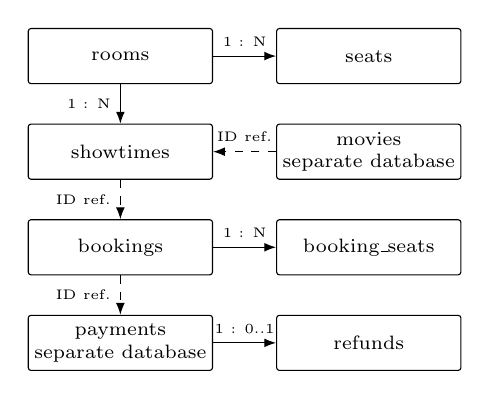
\begin{tikzpicture}[node distance=5mm and 8mm]
\node[box] (room) {rooms};
\node[box,right=of room] (seat) {seats};
\node[box,below=of room] (show) {showtimes};
\node[box,right=of show] (movie) {movies\\separate database};
\node[box,below=of show] (booking) {bookings};
\node[box,right=of booking] (bs) {booking\_seats};
\node[box,below=of booking] (payment) {payments\\separate database};
\node[box,right=of payment] (refund) {refunds};
\draw[arr] (room)--node[above,font=\tiny]{1 : N}(seat);
\draw[arr] (room)--node[left,font=\tiny]{1 : N}(show);
\draw[arr,dashed] (movie)--node[above,font=\tiny]{ID ref.}(show);
\draw[arr,dashed] (show)--node[left,font=\tiny]{ID ref.}(booking);
\draw[arr] (booking)--node[above,font=\tiny]{1 : N}(bs);
\draw[arr,dashed] (booking)--node[left,font=\tiny]{ID ref.}(payment);
\draw[arr] (payment)--node[above,font=\tiny]{1 : 0..1}(refund);
\end{tikzpicture}
\caption{Selected schema relationships reconstructed from SQL. Solid arrows
denote parent-to-child SQL foreign keys; dashed arrows denote logical ID
references. Reservations, identity, and other extension tables are omitted.}
\label{fig:data}
\end{figure}


Schema files and migrations are maintained in the initialized database
submodule, with additional backend SQL updates. The Compose initialization and
migration jobs mount these sources. Inspection verifies intended schema
structure and execution scripts, not successful migration of a running
database. No live data or production credentials were required or inspected
for the relational analysis \cite{deployment,db}.

\subsection{Payment and Asynchronous Follow-Up}
PayOS integration requests checkout links and queries payment status. Creation
includes merchant headers and an HMAC signature. The webhook path validates
the payload signature before trusting fields and checks order/amount against
the saved payment. A verified provider status can also trigger reconciliation
when the customer returns to the app. These source paths avoid equating an
external-browser launch with payment success \cite{booking,payos}.

Payment and booking records are not described as one distributed transaction.
The code contains a confirmation-or-refund path when payment succeeds after
the booking can no longer be confirmed. Staff record refund processing and
transfer references; automatic bank refund execution was not found. RabbitMQ
outbox workers publish persistent events after local commits, and consumers
process notification/refund and showtime-cancellation effects. Publisher
confirms and event-ID deduplication support retries but do not establish
exactly-once external email delivery \cite{booking,rabbit}.

\section{Mobile Application Architecture and Implementation}
\subsection{Startup and Navigation}
\code{main.dart} initializes Flutter bindings, creates the session object and
remote dependencies, attempts session restoration, and wraps the application
in \code{SessionProvider}. Unreadable storage is handled as a signed-out start.
Named routes create screens with their dependencies; an authenticated route
can redirect to sign-in with a pending destination \cite{client}.

The customer app exposes discovery, ticket history, notifications, and account
functions. Detail screens accept route IDs and reload data when an earlier
screen's argument is unavailable. This design also serves browser builds,
but on mobile it gives a consistent navigation contract without relying on
one global mutable booking object. It does not prove operating-system deep-link
registration or recovery of every transient form after process termination.
Table~\ref{tab:routes} lists representative route contracts.

\begin{table}[t]
\caption{Representative Mobile Screens}\label{tab:routes}
\centering\footnotesize
\begin{tabularx}{\columnwidth}{@{}lYY@{}}\toprule
Screen & Named route & Responsibility\\\midrule
Home & \code{/home} & Catalog and movie filters\\
Movie details & \code{/movies/\{id\}} & Metadata and showtimes\\
Seat selection & \code{/showtimes/}\allowbreak\code{\{id\}/seats} & Room layout and local choice\\
Summary & \code{/showtimes/}\allowbreak\code{\{id\}/summary} & Order options and submission\\
My bookings & \code{/bookings} & Ticket history\\
Booking details & \code{/bookings/\{id\}} & QR and lifecycle state\\
Payment & \code{/bookings/}\allowbreak\code{\{id\}/payment} & External checkout and checks\\
Notifications & \code{/notifications} & Read/unread messages\\
Profile & \code{/profile} & Account and member functions\\\bottomrule
\end{tabularx}
\end{table}

\subsection{Session State and Token Recovery}
\code{SessionState} is a \code{ChangeNotifier}, distributed through an
\code{InheritedNotifier}. It stores guest/authenticated state, user information,
expiration messages, and unread-notification count. Individual screens own
selection, loading, error, and pagination state. The code therefore uses a
small explicit state arrangement rather than an evidenced application-wide
Bloc or Redux architecture \cite{client}.

The HTTP client gives requests a default fifteen-second timeout and decodes
structured API failures. On a protected 401 it asks \code{TokenManager} to
renew the token, then retries once. Listing~\ref{lst:refresh} reproduces the
shared-future mechanism. Since the server rotates refresh tokens, independently
refreshing concurrent failed requests could otherwise reuse an invalidated
token. Additional session-version checks stop an in-flight renewal from
overriding a later account-expiration event \cite{client}.
\begin{lstlisting}[caption={Concurrent refresh coordination from TokenManager.},label={lst:refresh}]
return _pendingRefresh ??= _refresh(failedToken).whenComplete(() {
  _pendingRefresh = null;
});
\end{lstlisting}

Network errors can preserve session data for a retry; rejected refresh
credentials clear it. \code{SessionApp} responds to the expiration message by
opening sign-in and displaying an explanatory notice. This links transport
errors to navigation and prevents the UI from silently continuing with an
expired account state. It is an implementation mechanism, not evidence that
every race or device interruption has been exhaustively tested.

\subsection{UI Composition and Feedback}
Feature directories group authentication, movie, seat, booking, payment,
notification, profile, and staff screens. Shared theme files define spacing,
typography, color, and radius values. Reusable buttons, panels, loading,
empty, and error states keep common interactions consistent. Screen code uses
asynchronous calls, mounted checks, and busy flags to avoid updating disposed
widgets or repeatedly submitting an active action \cite{client,webui}.

The layout switches desktop navigation at 900 logical pixels, while phone
layouts use the narrow application frame. Seat maps and reusable column
components respond to available width rather than assuming a fixed desktop
canvas. The existence of phone-sized widget assertions supports testing those
layouts with fixtures; it is not a general accessibility, device-compatibility,
or performance certification.

\subsection{Platform-Specific Actions}
The native trailer implementation launches an external application rather than
embedding the browser-specific player. PayOS checkout likewise uses
\code{url\_launcher}. Ticket sharing invokes \code{share\_plus}, with clipboard
fallback on failure. Calendar support constructs a Google Calendar event URL;
it is not a synchronized device-calendar database integration \cite{client}.

QR ticket rendering uses \code{qr\_flutter}. A staff-only customer-app route can
look up a ticket or scan a QR through \code{mobile\_scanner}, then submit
server check-in. The iOS property list contains a camera-purpose description;
Android declares Internet access. Those inspected settings establish platform
intent, while camera permission behavior, release packaging, and physical-device
scanning remain unverified in this review \cite{client}.

\section{Core Business Workflows}
\subsection{Authentication and Account Use}
A customer may browse as a guest, but protected booking/account actions require
sign-in. Registration sends account data to AuthService and continues through
email OTP verification. Password recovery and profile editing have remote
service paths. Session restoration reads saved credentials and current-user
information; failures requiring authentication return the user to sign-in.
The application does not establish biometric login merely by depending on a
package that can support biometric options \cite{client,auth}.

\subsection{Discovery, Showtimes, and Seat Choice}
Home browsing combines now-showing/coming-soon selection, genres, and title
search, with a 350-millisecond debounce. Details expose metadata, trailer
actions, reviews, and open showtimes. The catalog repository fetches schedules
within a seven-day customer window. Once a show is chosen, room seats and
occupied IDs are combined into \code{ShowtimeSeatsData} \cite{client}.

The selected seat set remains local until order submission. A five-second
timer refreshes the visible map; conflicting local seats are removed, with
sweetbox partner handling. Failed refreshes retain the last map and retry on a
later tick. The booking transaction is consequently essential even when the
display recently looked current. This is periodically refreshed availability,
not verified WebSocket or SignalR push \cite{client,booking}.

\subsection{Order Calculation}
Summary collects seats, concessions, promotion choice, and requested member
points before submission. The backend recalculates the total. If $S$ is seat
value, $D$ the applicable ticket promotion, $C$ concessions, and $q$ redeemed
points, the code implements
\begin{equation}
T=S-D+C-1000q .\label{eq:total}
\end{equation}
The redemption ceiling is 50\% of the pre-points total and the account's
available balance. Promotion reductions are capped and rounded down to
1,000-VND steps. This notation explains real arithmetic rather than adding
an unrelated optimization model \cite{booking}.

Loyalty earning is also explicit. For paid amount $A$ and tier earn rate $r$,
the helper returns $\lfloor Ar/1000\rfloor$ points. The configured tier rates
are 5\%, 7\%, and 10\% for MEMBER, VIP, and VVIP. These values describe code
constants; no customer-retention or revenue effect has been measured.

\subsection{External Checkout and App Resumption}
Figure~\ref{fig:flow} describes the mobile checkout path. After creation of a
pending booking, the app requests a PayOS link and launches it externally.
\code{PaymentScreen} observes application lifecycle changes: a resumed app
that previously opened checkout requests verification. It also polls booking
state every five seconds, with provider verification every sixth eligible
poll, and disposes timers when leaving the screen \cite{client}.
\begin{figure}[t]
\centering
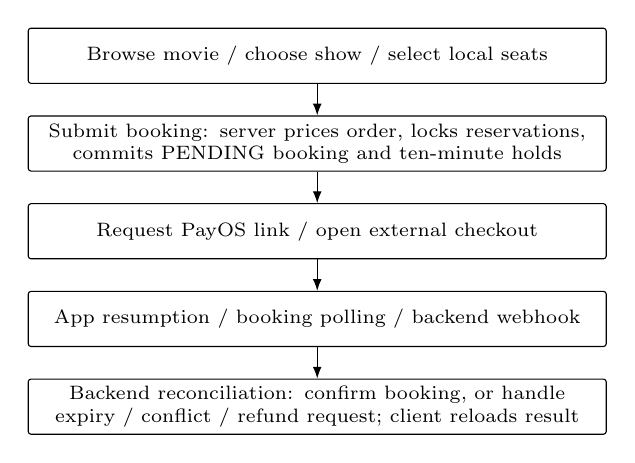
\begin{tikzpicture}[node distance=4mm]
\node[box,text width=72mm] (s) {Browse movie / choose show / select local seats};
\node[box,below=of s,text width=72mm] (b) {Submit booking: server prices order, locks reservations,\\commits PENDING booking and ten-minute holds};
\node[box,below=of b,text width=72mm] (p) {Request PayOS link / open external checkout};
\node[box,below=of p,text width=72mm] (v) {App resumption / booking polling / backend webhook};
\node[box,below=of v,text width=72mm] (r) {Backend reconciliation: confirm booking, or handle\\expiry / conflict / refund request; client reloads result};
\draw[arr] (s)--(b);\draw[arr] (b)--(p);\draw[arr] (p)--(v);\draw[arr] (v)--(r);
\end{tikzpicture}
\caption{Mobile external-checkout and resumption flow. No client redirect or timer is itself proof of payment.}
\label{fig:flow}
\end{figure}


The displayed countdown is computed from the booking expiry; it does not
authorize or extend the hold. A successful provider result is reconciled on
the backend before a confirmed ticket is shown. If the application is
terminated, booking history and ID-based detail loading provide a recovery
path; no claim is made that the OS automatically returns to the exact prior
payment screen or that offline purchase completion is supported.

\subsection{Tickets, Notifications, and Reviews}
Booking history/detail shows current status and paid-ticket QR content.
Sharing produces ticket text and a booking code; the QR must not be described
as cryptographically signed unless separately evidenced. Staff check-in
validates the booking on the server and records admission within a configured
time window. Review submission requires an owned booking that has been
checked in, with a unique user/movie review mapping \cite{client,booking}.

Notification lists retrieve stored messages and update read state through
APIs; the home/session UI tracks an unread count. Backend workers and event
handlers create reminder and ticket-related messages and send SMTP email.
No Firebase Cloud Messaging, APNs registration, or background OS push delivery
was established in the inspected implementation. Source-backed in-app records
and email must therefore be distinguished from native push notifications.

\begin{table}[t]
\caption{Major Mobile Functional Modules}\label{tab:modules}
\centering\footnotesize
\begin{tabularx}{\columnwidth}{@{}lYY@{}}\toprule
Module & Customer interaction & Supporting layer\\\midrule
Identity & Login, OTP, account recovery & Auth repository/AuthService\\
Discovery & Search, details, schedules & Catalog repository/MovieService\\
Reservation & Seats, options, summary & Booking repository/BookingService\\
Payment & External checkout, resumption & Payment screen/PayOS adapter\\
Tickets & History, QR, share, calendar URL & Flutter/native plugins\\
Messages & Lists, detail, read state & Notification APIs/SMTP handlers\\
Membership & Points, discounts, reviews & Booking business services\\\bottomrule
\end{tabularx}
\end{table}

\section{Security and Data Protection}
\subsection{Token and Account Protection}
The application persists access token, refresh token, expiry, and user data
using \code{SecureAuthTokenStorage}. It serializes writes and clears unreadable
storage. The package supplies platform-specific implementations
\cite{storage}; this review verifies calls to that abstraction, not hardware
backing or resistance to a compromised phone. No additional biometric gate,
certificate pinning, or device attestation was established \cite{client}.

Backend password/OTP hashing, input validation, role checks, and resource
ownership constrain API use. The booking controller replaces a customer's
submitted identity with claims, and price calculation uses backend data.
Gateway rate limiting and account-status validation add request controls.
These mechanisms reduce particular trust assumptions but do not establish
complete application security \cite{auth,gateway,booking}.

\subsection{Transport and External Data}
The default API addresses are HTTP development endpoints. HTTPS operation,
certificate configuration, and Android/iOS release network policies must be
verified for a named deployment. The client does not embed merchant signing
secrets in the inspected dependency construction; PayOS signing and webhook
checks occur in the backend. Actual secret values were not opened or printed
\cite{client,booking,deployment}.

Ticket sharing intentionally exposes booking information to the recipient.
Calendar actions construct an external URL containing event details. Those
flows should be explained to users in a release assessment rather than being
described as encrypted ticket distribution. Notification and payment records
also contain personal or payer metadata; no retention-policy or deletion
compliance guarantee can be derived solely from their entity definitions.

\section{Testing, Verification, and Evaluation}
\subsection{Executed Checks}
Table~\ref{tab:tests} records the review's verification outcomes. The installed
Flutter/Dart SDK and .NET SDK were identified directly. Backend isolated
tests succeeded: 17 BookingService unit cases and 21 gateway cases. AuthService
compiled with no warnings; MovieService compiled with four nullable warnings.
Gateway and BookingService builds also completed as part of their test runs.
These results do not measure device startup, frame rates, battery use, or
production API response times.
\begin{table}[t]
\caption{Verification Executed on October 28, 2026}\label{tab:tests}
\centering\footnotesize
\begin{tabularx}{\columnwidth}{@{}YY@{}}\toprule
\textbf{Check and method} & \textbf{Observed result / status}\\\midrule
BookingService isolated unit filter & \textbf{PASS}: 17 tests, zero failed\\
ApiGateway test project & \textbf{PASS}: 21 tests, zero failed\\
AuthService build & \textbf{PASS}: zero errors/warnings\\
MovieService build & \textbf{PASS}: zero errors; four nullable warnings\\
Flutter analysis & 1 informational lint; no errors/warnings\\
Flutter unit/widget suite & \textbf{PASS}: 209 tests after package restore\\
PostgreSQL/RabbitMQ integration suites & \textbf{BLOCKED}: Docker daemon unavailable\\
SQL/migration execution & \textbf{NOT EXECUTED}: no running database\\
Live PayOS, SMTP, deployed acceptance & \textbf{NOT EXECUTED}: external services not exercised\\
Native release/device verification & \textbf{NOT EXECUTED}: no device acceptance run\\\bottomrule
\end{tabularx}
\end{table}


After restoring the existing declared Flutter dependencies, the full
\code{flutter test --no-pub --reporter expanded} run passed 209 tests.
\code{flutter analyze --no-pub} reported one informational finding,
\code{curly\_braces\_in\_flow\_control\_structures}, in
\code{trailer\_url.dart:12}; no analysis errors or warnings remained.
The analyzer was therefore not a clean zero-finding run. The earlier
no-restore attempt failed because locally cached QR/sharing packages were
missing, and is not counted as a passed test run. No application source
was changed to obtain the restored-package result.
The shared client also compiled for its two browser entry points;
this does not substitute for Android or iOS release verification.



\subsection{What the Test Suite Can Establish}
Flutter tests cover model parsing, API-client handling, form validation,
navigation, seat maps, checkout states, account changes, ticket features,
and responsive views. They inject repositories, HTTP responses, and platform
substitutes. This accords with the distinction between unit/widget tests and
complete-device integration described by Flutter \cite{fluttertest,tests}.
Passing such tests does not demonstrate camera capture, an actual share sheet,
a real secure-storage backend, or banking completion on a physical phone.

Backend integration fixtures create PostgreSQL through Testcontainers and
can enable a RabbitMQ container; MovieService, PayOS, and SMTP are otherwise
substituted in the booking fixture. The Docker daemon was unavailable, so
those container suites and a full deployment were blocked. Database SQL and
mappings were inspected, but migrations were not run against a live database.
Android/iOS release builds and physical-device acceptance were not executed
\cite{tests,db}.

\subsection{Interpretation}
The evidence supports an implemented remote-client architecture and specific
tested backend helpers/policies. It does not support an overall mobile
acceptance rate, production availability, a completed merchant transaction,
or a quantified security level. A workflow with both UI code and API code is
reported as implemented in source with runtime verification outstanding where
appropriate. No fixture data or example payment record is counted as a
successful real customer action.

\section{Limitations and Future Development}
\subsection{Current Limitations}
The client depends on connectivity for catalog retrieval, booking, and payment
confirmation. A stale seat map is possible between polling ticks or after a
failed refresh. External checkout introduces operating-system lifecycle and
browser behavior that widget mocks cannot fully reproduce. The implementation
does not establish offline booking, native push, universal app links, or
biometric authentication merely through route names or dependencies
\cite{client}.

Refund transfer remains manual staff work. Email sending and database updates
are separate operations despite event-ID checks, so exactly-once SMTP delivery
is not guaranteed. Local-time timestamps with Npgsql legacy behavior constrain
assumptions about users in other time zones. The source includes a calendar
duration fallback of 150 minutes when exact showtime data cannot be obtained;
that fallback is a convenience, not guaranteed schedule accuracy
\cite{booking,client,deployment}.

The review could not demonstrate live provider operation, container integration,
native secure storage, QR scanning, or signed store distribution. Existing SQL
seed payment labels are demonstration data, not evidence of active VNPAY or
MOMO implementations. Platform folders establish potential targets rather
than a tested support matrix. These limits prevent describing the application
as production-ready.

\subsection{Recommendations}
Recommended next steps are a controlled Android/iOS device matrix, release
build and permission checks, and lifecycle tests that interrupt checkout at
multiple stages. Verification should include token restoration after process
death, network transitions, camera denial, share-sheet failure, and repeated
payment reconciliation. Container suites and schema migrations should be run
before a complete system acceptance test.

Further recommendations include validating HTTPS and release network policy,
testing accessibility and text scaling, resolving backend nullable warnings,
and reviewing notification delivery requirements before considering native
push. Any push, offline cache, biometric gate, or deep-link enhancement should
be treated as proposed development rather than an implemented feature or
committed project roadmap.

\section{Conclusion}
CosmoQ's mobile implementation provides a Flutter customer workflow over a
shared ASP.NET Core backend. Session recovery, remote repositories, periodic
seat updates, server-created holds, external checkout reconciliation, and QR
ticket access form the central implementation. SQL constraints and backend
authorization carry responsibilities that cannot safely be delegated to phone
UI state. The reported verification establishes selected compilation and
automated-test outcomes while preserving the gap to physical-device and live
provider validation. The system is therefore documented as an implemented
mobile client with explicit operational verification limits.
\section*{Acknowledgment}
The student developers thank Mr. Huynh Vang, Department of Software Engineering,
FPT University Quy Nhon Campus, for his guidance as project advisor and for
supporting the team's software engineering work on CosmoQ Cinema.
\balance
\bibliographystyle{IEEEtran}
\bibliography{references}
\end{document}
